\documentclass[onecolumn, draftclsnofoot,10pt, compsoc]{IEEEtran}
\usepackage{graphicx}
\usepackage{url}
\usepackage{setspace}

\usepackage{listings}
\usepackage{xcolor}

\usepackage[T1]{fontenc}
\usepackage[scaled]{beramono}

\usepackage{pdfpages}

\usepackage{color}
\definecolor{bluekeywords}{rgb}{0.13,0.13,1}
\definecolor{greencomments}{rgb}{0,0.5,0}
\definecolor{redstrings}{rgb}{0.9,0,0}

\lstset{language=[Sharp]C,
showspaces=false,
showtabs=false,
breaklines=true,
showstringspaces=false,
breakatwhitespace=true,
escapeinside={(*@}{@*)},
commentstyle=\color{greencomments},
keywordstyle=\color{bluekeywords}\bfseries,
stringstyle=\color{redstrings},
basicstyle=\ttfamily
}

\usepackage{geometry}
\geometry{textheight=9.5in, textwidth=7in}

% 1. Fill in these details
\def \CapstoneTeamName{			Velocity-Raptors}
\def \CapstoneTeamNumber{		37}
\def \GroupMemberOne{			Alex Bailey}
\def \GroupMemberTwo{			Dylan Washburne}
\def \GroupMemberThree{			Benjamin Wick}
\def \CapstoneProjectName{		Object Velocity Tracking}
\def \CapstoneSponsorCompany{}
\def \CapstoneSponsorPerson{		Alex Neighbors}

% 2. Uncomment the appropriate line below so that the document type works
\def \DocType{		%Problem Statement
				%Requirements Document
				%Technology Review
				%Design Document
				Final Report
				}
                

\usepackage{listings}
\usepackage{color}

\newcommand{\NameSigPair}[1]{\par
\makebox[2.75in][r]{#1} \hfil 	\makebox[3.25in]{\makebox[2.25in]{\hrulefill} \hfill		\makebox[.75in]{\hrulefill}}
\par\vspace{-12pt} \textit{\tiny\noindent
\makebox[2.75in]{} \hfil		\makebox[3.25in]{\makebox[2.25in][r]{Signature} \hfill	\makebox[.75in][r]{Date}}}}
% 3. If the document is not to be signed, uncomment the RENEWcommand below
\renewcommand{\NameSigPair}[1]{#1}

\definecolor{mygreen}{rgb}{0,0.6,0}
\definecolor{mygray}{rgb}{0.5,0.5,0.5}
\definecolor{mymauve}{rgb}{0.58,0,0.82}

\lstset{ %
  backgroundcolor=\color{white},   % choose the background color
  basicstyle=\footnotesize,        % size of fonts used for the code
  breaklines=true,                 % automatic line breaking only at whitespace
  captionpos=b,                    % sets the caption-position to bottom
  commentstyle=\color{mygreen},    % comment style
  escapeinside={\%*}{*)},          % if you want to add LaTeX within your code
  keywordstyle=\color{blue},       % keyword style
  stringstyle=\color{mymauve},     % string literal style
}

%%%%%%%%%%%%%%%%%%%%%%%%%%%%%%%%%%%%%%%
\begin{document}
\begin{titlepage}
    \pagenumbering{gobble}
    \begin{singlespace}
    	
\includegraphics[height=4cm]{coe_v_spot1}
        \hfill 
        % 4. If you have a logo, use this includegraphics command to put it on the coversheet.
        %\includegraphics[height=4cm]{CompanyLogo}   
        \par\vspace{.2in}
        \centering
        \scshape{
            \huge CS Capstone \DocType \par
            {\large\today}\par
            \vspace{.5in}
            \textbf{\Huge\CapstoneProjectName}\par
            \vfill
            {\large Prepared for}\par
            \Huge \CapstoneSponsorCompany\par
            \vspace{5pt}
            {\Large\NameSigPair{\CapstoneSponsorPerson}\par}
            {\large Prepared by }\par
            Group\CapstoneTeamNumber\par
            % 5. comment out the line below this one if you do not wish to name your team
            %\CapstoneTeamName\par 
            \vspace{5pt}
            {\Large
                \NameSigPair{\GroupMemberOne}\par
                \NameSigPair{\GroupMemberTwo}\par
                \NameSigPair{\GroupMemberThree}\par
            }
            \vspace{20pt}
        }
        \begin{abstract}
        % 6. Fill in your abstract    
        	This document is the final written document for our capstone project. It will give an overview of everything we did this year.
            
        \end{abstract}     
    \end{singlespace}
\end{titlepage}
\newpage
\pagenumbering{arabic}
\tableofcontents
% 7. uncomment this (if applicable). Consider adding a page break.
%\listoffigures
%\listoftables
\clearpage

% 8. now you write!
\section{Introduction}
This project was requested by our client Alex Neighbors.
This was a personal project the he had envisioned.
The goal was to create a proof of concept of an alternative method of speed tracking.
In our case, our alternative was a video camera. Specifically, the Microsoft Kinect.
The members of the team included Alex Bailey, Dylan Washburne, and Benjamin Wick.
We all had similar roles in the project however, we all specialized in different areas when contributing. Alex focused on hardware connectivity and the speed algorithm. Dylan's main focus was the speed algorithm. Finally, Ben focused on the computer vision library and object tracking.
Our client Alex, played the role of our supervisor and was there to help along the way.

\newpage
%%%%%%% WE NEED TO PUT ORIGINAL REQUIREMENTS DOCUMENT HERE %%%%%%

\section{Requirements Document}
(Begins on next page.)
\newpage

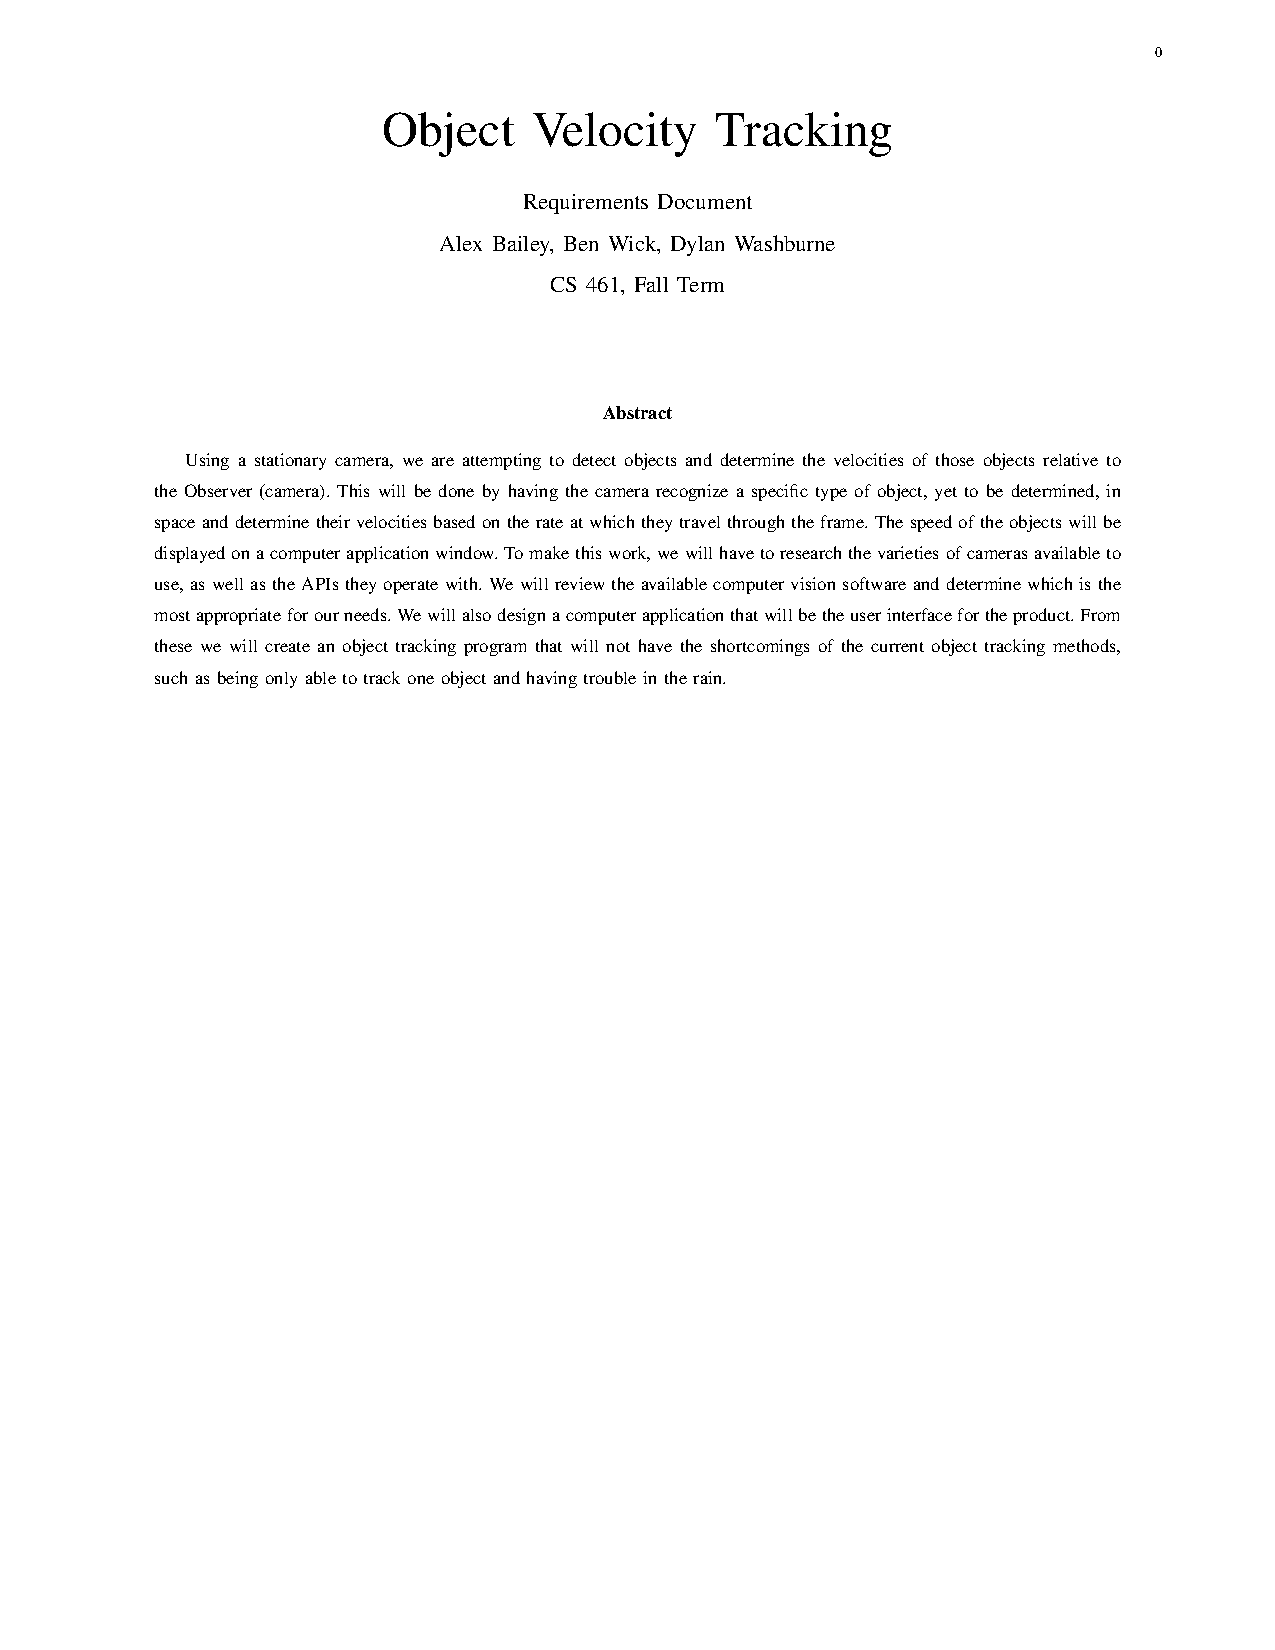
\includepdf[pages={1-}]{requirements.pdf}

\subsection{Changes Made}
\begin{tabular}{|p{0.075\linewidth} |p{0.25\linewidth}|p{0.25\linewidth}|p{0.25\linewidth}|}
\hline 
Number & Requirement & What happened to it & Comments \\
\hline 
1 & Track multiple objects & Changed to single object & Our client informed us that this project was intended on being a proof of concept. We decided to first focus on tracking one object at a time. \\
\hline
2 & Work up to 100 meters & Changed to 10 meters & At first we were unaware that depending on our camera we would be very limited. We ended up using the Microsoft Kinect which has a max range of 10 meters. \\
\hline
\end{tabular}
\subsection{Final Gantt Chart}
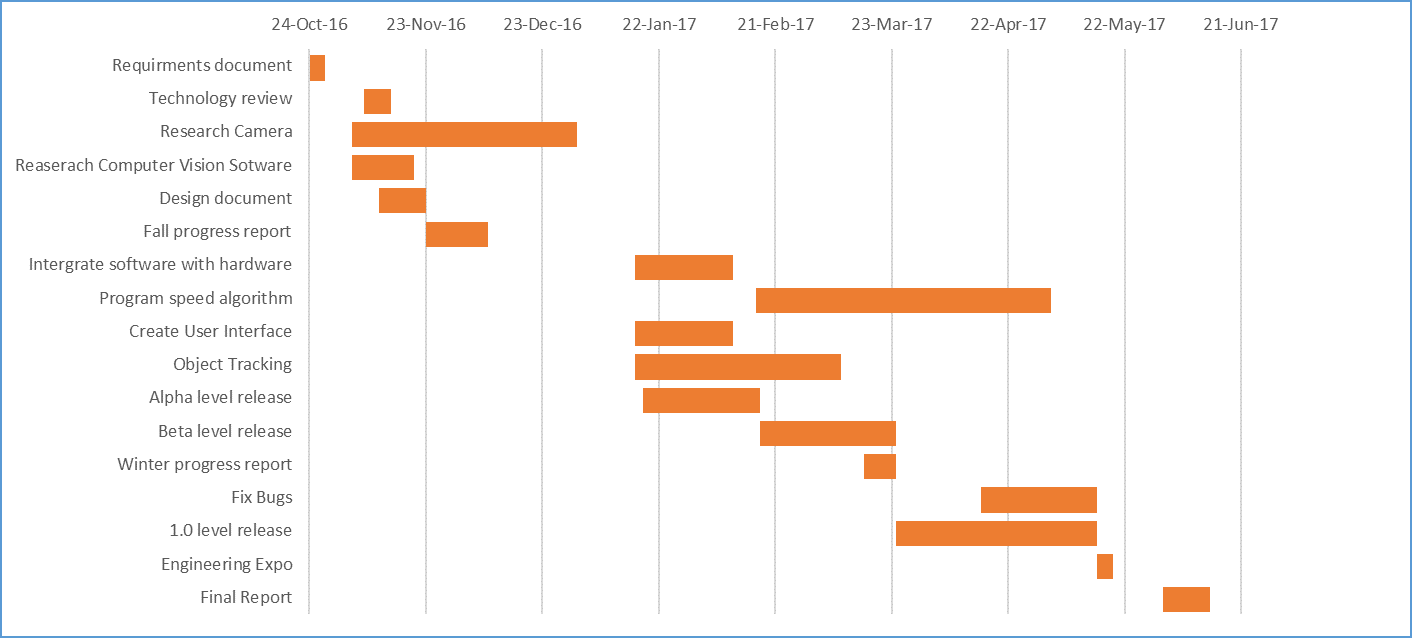
\includegraphics[scale=.80]{gantt2}

%%%%%%% WE NEED TO PUT ORIGINAL DESIGN DOCUMENT HERE %%%%%

\newpage
\section{Design Document}
(Begins on next page.)

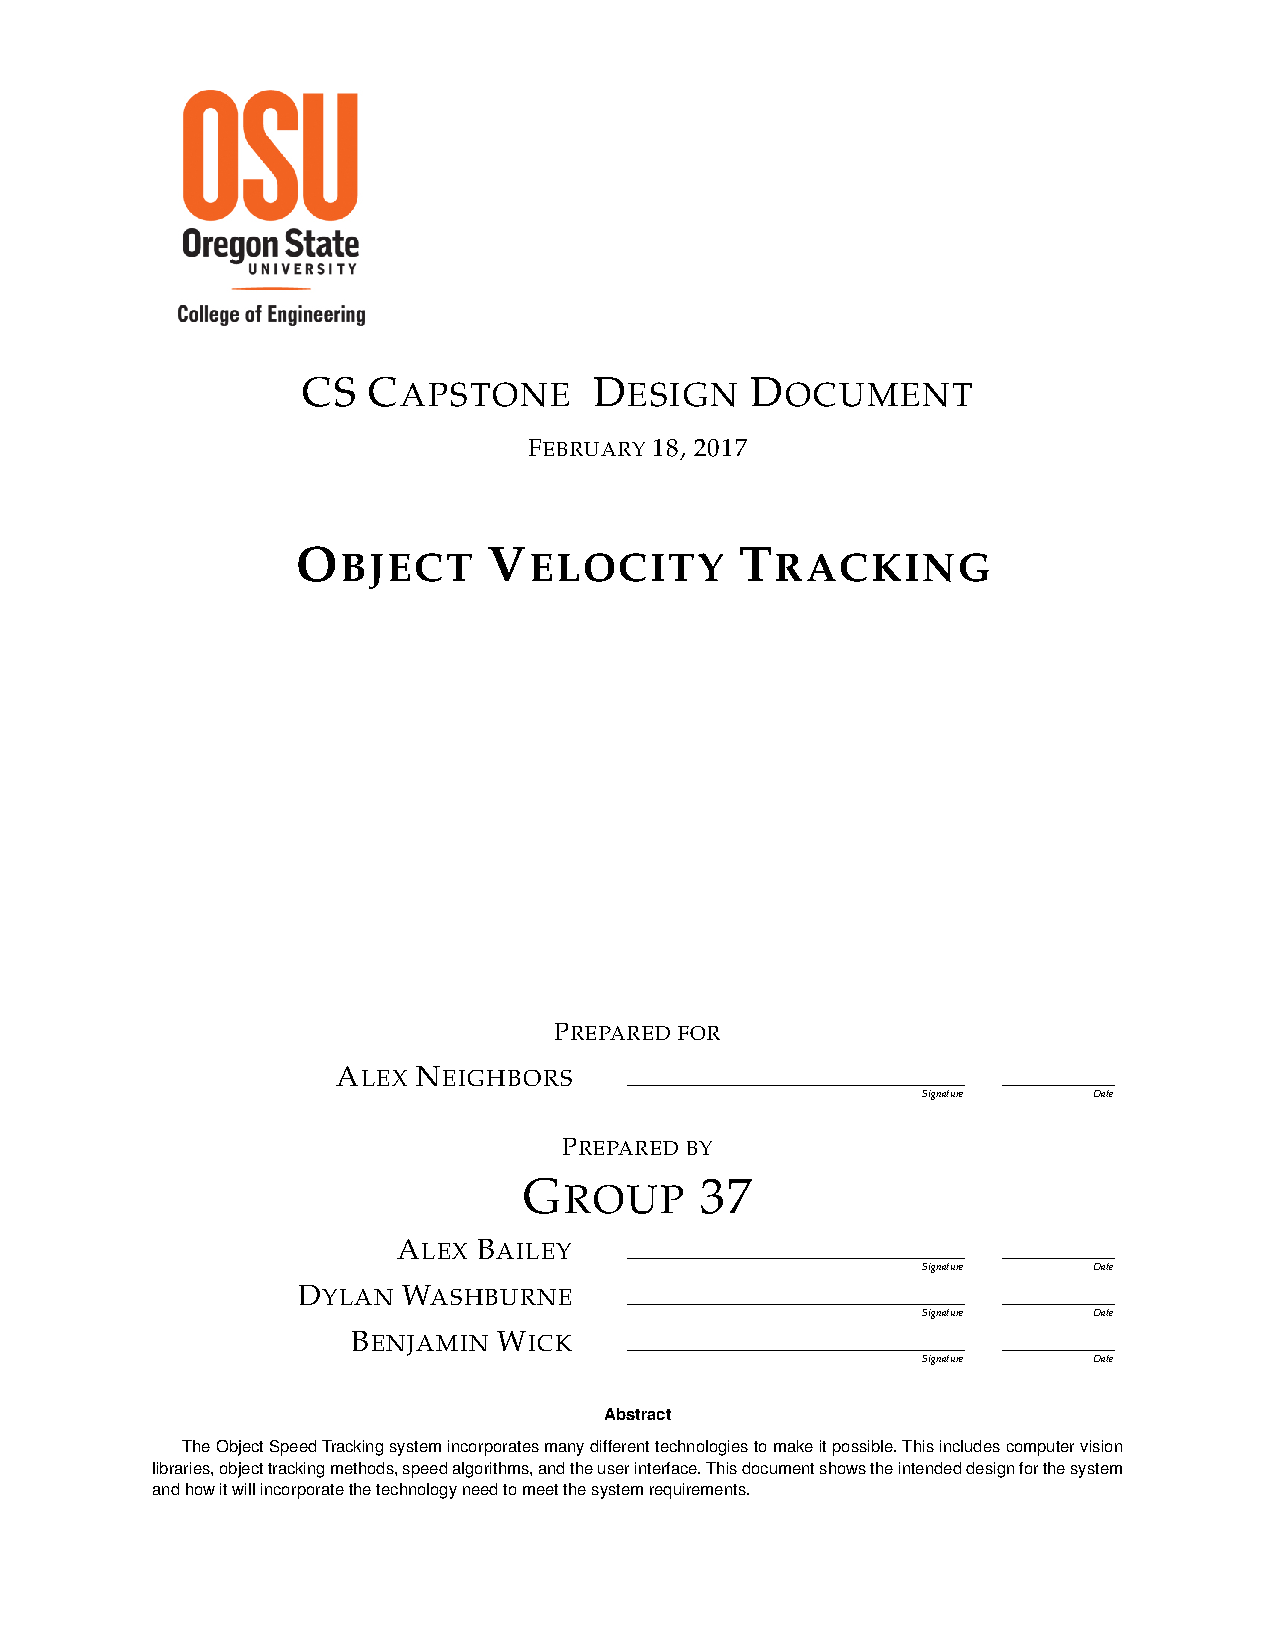
\includepdf[pages={1-}]{design-document-revised.pdf}

\subsection{Changes Made}

In this document there were some changes from the original design to the final.
The recording and replay feature changed a significant amount.
Firstly, our final application cannot replay the video.
Secondly, instead of saving the recordings as video, the recordings are saved as images.
Thirdly, the recordings are not saved in a structured database as originally intended, but are saved to a specified file that they could be view from.
Another change from the original is the accuracy of the speed.
Originally we planned on 90\% accuracy, but this was difficult to verify as the objects we tested rarely had a consistent speed.
Therefore the accuracy of the speed is likely lower than 90\%.
Another difference in this document is that we changed from multiple objects to a single object.

%%%%%%% WE NEED TO PUT ORIGINAL TECH REIVEW DOCUMENT HERE %%%%%%


\newpage
\section{Tech Review}
(Begins on next page.)

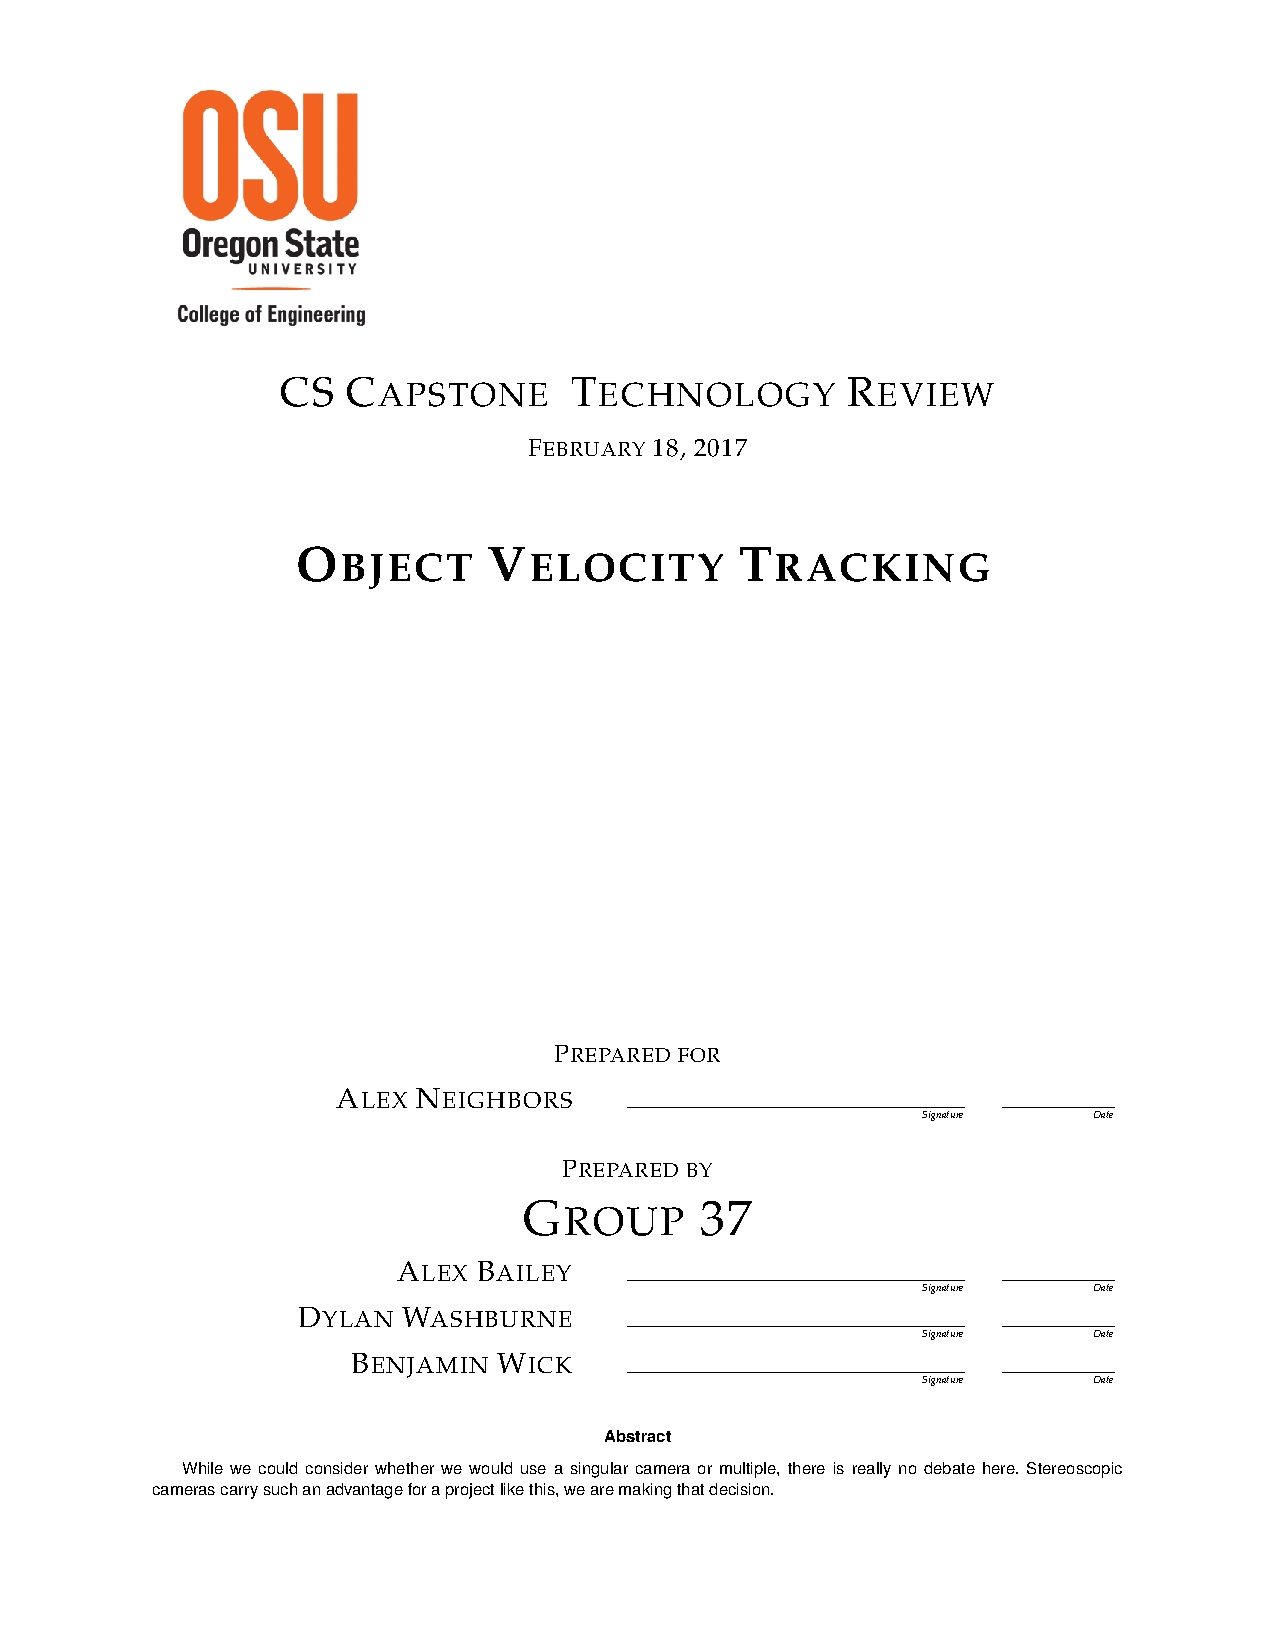
\includepdf[pages={1-}]{tech-review-document.pdf}

\subsection{Changes Made}
For object tracking we listed several different methods. We ended up choosing to use a simpler approach for tracking because the object was changed to a red ball. Our other options included haar cascades, background subtraction, and SURF. Looking further into using haar cascades, a lot of sources online discouraged the use of it for simple objects like a red ball. The method would have involved us to track certain features of the object but because the red ball is simple enough it would have been essentially a color tracking method. This is also the same reasoning against using the SURF detection method. The last option, background subtraction, was also considered. However, we wanted our project to work without a pre-determined background which is why we decided not to use this.

Another Change made was not using any of the long term storage methods talked about which includes AVI, MP4 and MKV video storage. In the initial design we intended it on being saved as a video. In our final completion, however, we used images and decided to save the images instead.

We also altered the velocity formula we were to include from the tech review document.  In the tech review, we looked at several sophisticated methods for extracting velocity from an object on-screen, however in the end it turned out that we didn't need a method that was sophisticated so much as a method that worked.  Given our resources at hand, it made more sense to simply take the translation of the object's position as a vector and use that vector as the velocity.



\section{Weekly Blog Posts}
\subsection{Alexander Bailey}
\subsubsection{Fall Term}

\textbf{Week 3}
\newline
Our progress so far is that we have talk to our client and discussed what he wanted for the project and made a problem statement that he and our group agree on.\newline
For next week, we will begin looking into the different types of cameras that are available and their APIs to determine which type of camera and API will best suit our needs. We will also research the various programs that currently exist that are related to our problem and how much our group will need to do from scratch.
Currently there have been no problems.
\newline
\textbf{Week 4}
\newline
This last week I gave an update to our client about the need to redo the problem statement and the impending requirements document. I emailed our TA asking for comments on our problem statement.
\newline
For this coming week, we are going to get our problem statement revised. We are meeting on Monday to work on the requirements document.
\newline
We haven't had any problems
\newline
\textbf{Week 6}
\newline
This week, we polished up our requirements document with feedback from our TA Jon Dodge and Professor Kirsten Winters. We are sending our client the requirements document for his input and signature. Next week we will be writing out tech reviews. There were no problems.
\newline
\textbf{Week 7}
\newline
This week we got approval from Alex Neighbors on our Requirements Document and submitted it. We also discussed our Tech Review and did some research.
\newline
Next week, we will finish up the Tech review and begin working on our Design Document.
\newline
One problem with this week is that we had not figured out what 9 things we were going to do for our Tech Review.
\newline
\textbf{Week 8}
\newline
Last week we wrote our tech review and got started on the design document
\newline
This week we will be continue to work our design document.
\newline
There were no problems this week.
\newline
\textbf{Week 9}
\newline
This week we began work on the design document.
\newline
Next week we are going to finish up with the design document and begin writing our progress report.
\newline
There were no problems this week.
\newline
\textbf{Week 10}
\newline
This last week we wrote the Design document.
\newline
Next week we are going to write the progress report and record it.
\newline
There were no problems.
\newline
\textbf{Week 11}
\newline
Due to Finals we did not do much work, but we did get our paper approved by Alex Neighbors.
\newline
In the next few weeks we intend to choose a camera.
\newline
We had no problems this week.

\subsubsection{Winter Term}

\textbf{Week 2}
\newline
This week we are having Alex Neighbors send us the Zed camera. I also began learning C\#.
\newline
Next week we will continue to learn C\# and making a GUI.
\newline
No problems to report.
\newline
\textbf{Week 3}
\newline
This week we continued learning C\#.
\newline
Next week the camera should have arrived and we can begin testing it out.
\newline
No problems this week
\newline
\textbf{Week 4}
\newline
This Week we received the Xbox 360 kinect camera and are waiting on the usb adapter to begin testing with it. We also are making the skeleton for the GUI.
\newline
Next week we should have the adapter and can begin working with the kinect. Next week we plan to be able to view a camera within our GUI.
\newline
No problems.
\newline
\textbf{Week 5}
\newline
This week we received the USB adapter for the Kinect camera, so we can begin using it. I looked further into using image subtraction for tracking.
\newline
Next week I'll look more into using the Kinect with C\#.
\newline
No problems.
\newline
\textbf{Week 6}
\newline
This week we worked on updating the documents for the alpha level release.
\newline
Next week I'll continue looking into Kinect.
\newline
no problems.
\newline
\textbf{Week 7}
\newline
This week I worked on getting the depth map to display on the screen.
\newline
Next week, I'll continue working on the depth map.
\newline
No problems this week.
\newline
\textbf{Week 8}
\newline
This week I got the depth map to display as a black and white screen, however the screen oscillates for some reason. More specifically as an object moves towards and away from the camera the object should move from black to white with white being closest and black being far way, but instead it the object will go black then white then black then white, etc.
\newline
Next week I will try and find out why the depth map is doing this.
\newline
No problems this week.
\newline
\textbf{Week 9}
\newline
This week I worked on fixing the depth map so that it doesn't cycle between black and white.
\newline
Next week I will continue to work with the depth map.
\newline
No problems this week.
\newline
\textbf{Week 10}
\newline
This week we mainly focused on the poster and progress report paperwork, so little was done on the actual project. We got confirmation to use colored balls for tracking and to scale back the recording and replaying feature.
\newline
Next week we will continue working on the paperwork.
\newline
No problems.

\subsubsection{Spring Term}

\textbf{Week 2}
\newline
This week we were able to get the object tracking working with the Kinect camera and began working on getting the depth data at a specified point.
\newline
Next week we will finish adding the finding depth of the center of the object.
\newline
One problem that we aren't entirely sure about is that if too much red enters the frame then the camera will not update, but as soon as the red leaves the frame, the camera is fine. Luckily, it works fine when only one ball of red is in the frame, so this will work for our needs, but we are also looking into Haar cascades, which would hopefully remove this problem.
\newline
\textbf{Week 3}
\newline
This week we mainly worked on a surprising error where only Ben's computer was able to run the Kinect. We also had the poster review session with professor Kirsten and were able to get some good feedback.
\newline
Next week we will probably abandon trying to fix the error due to the limited amount of time till the code freeze. Instead we will focus on the speed algorithm.
\newline
Currently we have the problem that we fear that we may not have enough time to complete all the things in our requirements document, such as the recording an play back, so we will talk to our client in order to identify the most important aspects of the project.
\newline
\textbf{Week 4}
\newline
This week we were able to get speed tracking working and displaying in a text box. We also made a final draft of the poster and had it approved by our client.
\newline
Next week we're going to get recording and the text output file working, should be in time for the Code freeze.
\newline
The only problem we had is that for some reason my computer has trouble running the recording software, whereas my teammates computers don't seem to have a problem. Mine will show the text of the balls position but won't show the video. However, if I remove enough code from our speed tracking function, it will show up.
\newline
\textbf{Week 5}
\newline
This week we tested the speed function. We also had the program output a text file of the data. We also started the recording process, but for some reason this caused problems with the live feed.
\newline
Next week we are going to work on the midterm report and recording feature.
\newline
No problems.
\newline
\textbf{Week 6}
\newline
This week we began the midterm report paper and video.
\newline
Next week we are going to finish our report and then we are going to make sure that our project is ready for the expo display and record a video in case we have trouble doing a live demo during expo.
\newline
No problems.
\newline
\textbf{Week 7}
\newline
This week we finished the paperwork for the progress report, made a demo for expo, and went to expo.
\newline
Next week we are going to start the 3 writing assignments.
\newline
No problems.
\newline
\textbf{Week 8}
\newline
This week we contacted our client about the final hand off and returning the kinect.
\newline
Next week we'll begin work on the final documents.
\newline
No Problems.
\newline
Extra Questions
\newline
If I were to redo this project from the fall term, I would tell myself to not be so ambitious in the design of the document.
\newline
Getting experience with C\# is definitely big. Secondly would be working with a openCV.
\newline
Mainly the C\# for GUIs, but possible openCV if I get into some kind of computer vision.
\newline
I liked the interactive nature of the project, it was fun to see the program recognizing objects as they were in motion.
\newline
My teammates taught me about openCV and finding the speed of the object in 3D space, as that was the pieces they were in charge of.
\newline
I might possibly be disappointment given the original design, but knowing more about object recognition and tracking I think I would be okay knowing that the students had no prior experience with it.
\newline
The next step would probably be multiple object tracking.
\newline

\subsection{Dylan Washburne}
\subsubsection{Fall Term}

\textbf{Week 3}
\newline
Since the start of the term, we have now been assigned into this project group, spoken with our client, and determined what we are going to be doing in the project. Personally, I attribute almost all of this to preparing the Project Statement, though honestly it had to be done eventually.
\newline
In the upcoming week, we will be researching the available varieties of cameras that would be applicable to this project. This involves researching which cameras can be most effectively used to capture real-time data, as well as determining if we want mono- or bi-focal cameras.
\newline
We are also looking into the apis used in the programming of these cameras. While not determined as of yet, we have discussed the point and believe looking into what cameras already have the capability to recognize objects in the frame is a serious consideration to work with.
\newline
\textbf{Week 4}
\newline
In the last week, I've mostly been looking up some camera options in my free time. The issue with doing this without dedicating serious time to it is that it's a little difficult to locate all the information pertaining to the coding side, and whether or not it has built-in capability to locate objects in frame. Granted, certain cameras like Kinect heavily emphasize that point, but I'm going to need to look a lot more at the api side of things to see if it will behave as needed for this endeavor.
\newline
In the coming week, I'm planning on getting the problem statement fully revised, as well as typing out the requirements document. I also hope that the group can sit down and definitively decide what camera we're going to use, because that's going to be needed soon when we are able to begin the actual work.
\newline
\textbf{Week 5}
\newline
This last week was kind of hectic, but due to a lot of factors not directly influenced by this class. Apart from us redoing the problem statement and making a requirements document, I also had 2 midterms on the same day, so you know... everything suffered just a bit.
\newline
On a happy note, now that we've got all this out of the way we can finally start actually doing hard work on the project. And yes, this means actually selecting a camera to use, just as I said 3 weeks ago. That has been our client's number one request to us and we haven't been able to do it very well due to mass overlap in time where we can be together, and documents that need to get done.
\newline
\textbf{Week 6}
\newline
This week was terrible for me because of non-capstone reasons. As far as capstone itself goes, this week was fairly uneventful, as we mostly did edits to the requirements document. I did personally look a little into cameras and object tracking, but I still have no concrete idea what would be best overall for our purposes.
\newline
We really need to get the type of camera locked down. Whatever work we get next week is hopefully trivial so we can, as a group, come together and finally research that.
\newline
\textbf{Week 8}
\newline
This week was a nice slap in the face to me for our writing. A lot was done between Sunday and Wednesday to make the tech review actually happen. For me, though, I most hustled in redoing our citations, and even that I know wasn't properly done, since /cite didn't want to work for me.
\newline
Upcoming, more documents to be done. Yay, more writing! Sorry that was sarcastic, but it's how I deal with being mad at myself over the last week. Writing isn't particularly hard, and I see the applications to all the assignments, so I don't really mind the writing all that much.
\newline
\textbf{Week 9}
\newline
This last week was Thanksgiving week, so not much time was devoted to this work. Nonetheless, we now have divided up the work for our upcoming document.
\newline
Going forward, we will complete that document for real.
\newline
Seriously, not much to say this week.
\newline
\textbf{Week 10}
\newline
The previous week was mostly us completing the requirements document. This took less time than anticipated, but only because it required us to understand everything before we could actually start, which means the combined time was much longer. We also did a little work towards the progress report, but there's still a long way to go on that.
\newline
Coming up, we must finish the progress report. After that, we can actually begin on the project itself over winter break. I anticipate we will group a little, but much of what we have to do requires all of us here. Our first steps to get setup complete I anticipate will take a few weeks.

\subsubsection{Winter Term}
\textbf{Week 1}
\newline
Winter break didn't really do anything for our project's completion, since we didn't meet up. We all seem to remember everything with good detail though, so there was no loss either.
\newline
We have researched stereoscopic cameras, and found that the market is somewhat cornered to models which have a maximum range of 20m. In fact, most only reach about 3m away, because the major market is peoples' living rooms. Our initial goal of 100m is not going to happen unless we construct it ourselves. That said, we have reevaluated how much we need to track every object in a football stadium, and while a bit more range would be welcome, 20m would satisfy our needs well. We are hoping we can update our requirements to reflect that.
\newline
\textbf{Week 4}
\newline
We have received the camera to work with. It was not the Zed as we had proposed, but rather a Kinect. I am cautiously optimistic about this change in scope, because narrowing it down is actually a good thing, so we are constrained by force to not over-deliver what we can't possible create.
\newline
I kind of wish we had heard the context for this selection from Alex before he sent it to us, but he's explained it now and we all understand. We just sort of wish we had heard this context before we got the package and were rather confused.
\newline
We need to do a loot in the coming weeks to get our alpha product done, but I'm hopeful we can get a compact starting product prepared. Unpolished maybe, but I think it can be done.

\subsubsection{Spring Term}
\textbf{Week 2}
\newline
In the previous week, we had a good number of new developments. We were able to make the object tracking perform correctly for objects with the color red, and we have begun implementing that alongside the depthmap. The implementation to make it coincide with the depthmap is not yet complete, but quite frankly at this point the progress we have made is good enough for me.
\newline
The main difficulty here is that we are still moving slower than we should, for our point in the term. We have accepted that and been working hard to try and approach where we need to be.
\newline
Coming up, we are preparing to update our poster for expo (and the assignment where we need to update it), as well as once again sending a message to our client on how we are modifying the project requirements.
\newline
\textbf{Week 3}
\newline
This week we received some small red stress balls to work with as objects for the video to focus on. They appear to work well enough, although there are still some issues inherent in the program. We are hoping to resolve them well enough for our expo presentation to be workable.
\newline
We also did poster reviews for extra credit in Kirsten's office. To be frank, we knew our poster was a bit terrible going in. That said, we got extremely good feedback from the other group on how specifically to improve the poster. I feel we can make it look good by expo, so I am happy with the meeting.
\newline
I am still worried that we may not be able to fix everything by expo. I don't exactly have a plan for us being unable to do this, but it is my largest current concern for this project.
\newline
\textbf{Week 4}
\newline
This week, we completed a method to take the xy coordinates in the color image, the image which does the object recognition and tracking, and use those coordinates to look up the z distance away from the camera through the corresponding coordinates in the depthmap. This allows us to automatically locate the center of an object, and determine its precise point in space every frame.
\newline
From there, I was able to integrate some formulas to calculate velocity, half through knowing the Pythagorean theorem, and half through fiddling with data of a tracked ball at various depths to understand how many pixels it translates horizontally, based on its distance from the camera. Naturally, an object farther away travels fewer pixels horizontally than an object up close, when translating the same distance in the real world.
\newline
Coming up, we still need to hammer out a few issues before the code freeze. We are also actively working on touching up the poster before it gets turned in. We have already gained client approval, but we are looking for more minor isues at this point like visual spacing of text boxes (and only to a minor degree, nothing that would change the poster in any significant manner).
\newline
\textbf{Week 5}
\newline
Code freeze hit on Monday. We were working nearly until the deadline to submit what we felt could be a "complete" product. Granted, we completed most everything before this point, but the last-minute things were more of the small-scale issues which we felt should be featured in a "release".
\newline
We also submitted the poster and completed all the individual paperwork required to present at the expo. It was really just busywork, so it was completed in good time.
\newline
Since the code freeze hit and we have essentially "submitted" our project, we have actually let ourselves not meet up as often this week. I believe this to be a temporary measure, partially because there are also midterms, but we will be working again to complete the grading assessment paperwork before that is due. We plan to meet over the weekend to bang most of that out.
\newline
\textbf{Week 6}
\newline
No major breakthroughs have happened this week. To be brutally concise, we have not worked on the actual project in any significant capacity. This is mostly because of other events in each of our lives, notably midterms. It is also notably because we have been working on the "midterm" progress report.
\newline
The midterm still has to be completed. We are catching back up on the paperwork to reflect our actual state of affairs, relative to the previous progress report last quarter. Unlike the last 6 months, we actually have a product to show off for this. This will likely lead to more time spent making the video, to represent what has been completed.
\newline
\textbf{Week 7}
\newline
Expo happens this week. I think we are as prepared as we will ever be, and I'm honestly just waiting for it to be over. I am sure within 90\% tolerance that it will go smoothly, with probably a couple of people causing minor trouble, but nothing show stopping.
\newline
\textbf{Week 8}
\newline
Expo was last week. Overall I would say it went about as well as expected, though I do wish in retrospect I had packed some different shoes, more aligned to standing in place. Since then, we have not met up in any major capacity regarding capstone, even though we still meet for other class projects. I don't know about Alex and Ben, but I think we are all fairly satisfied with how the expo went.
\newline
Looking back, there are a number of things I would have done differently this term. For whoever is reading this, this is where I am beginning the retrospective questions.
\newline
If I were to redo this from the fall term, I wouldn't change much from the fall term until we hit the requirements document. There, I would say that we should have promised way less. Of course, we slashed it down to a moderate size as time passed, which I would also say is the biggest thing I learned. I never before realized how often people in the industry would have to go back and tell the client they were cutting features.
\newline
In the future, I can see myself using a number of the delegation skills I honed over this term. My programming skills weren't really the largest factor over the project, though I did learn a few new things. Rather, the ability to work with the team and figure out the work loads was the most important skill I had to use nearly every time we met. I suppose you can also say this is what I learned from my teammates, because I can confidently say that all of my notable gains in skill from this project came from interacting with the team.
\newline
I liked that the project was truly us building an application from the ground up, with no preexisting code base, though that's a double edged sword because I know any job I acquire will want me to implement on an existing system instead of building my own, and I would have preferred to work on something existing so I could get more real experience.
\newline
If I were the client for the project, I am not sure if I would be satisfied with the work done. On the one hand, we delivered a working proof-of-concept at the quality you might expect from recruiting random college undergrads who have never had a job, but simultaneously we could have created something of higher quality that runs better with better market applications. Though, I also think the project itself wasn't exactly that aimed at top-end market applications anyway.
\newline
Were this project to be continued next year, I think they could get good progress by optimizing the object recognition algorithm because that's where all the processing is going, and from there expanding the objects it can recognize. They could even scale up to a higher quality camera with higher range to expand the applications the product would be viable in.


\subsection{Benjamin Wick}
\subsubsection{Fall Term}
\textbf{Week 3}
\newline
This week we learned a lot more about our project. We did some research on cameras that we might use for our project. We also worked on our abstract and problem statement. Next week, we plan on continuing our research and hope to come up with a list of possible cameras we can use.
\newline
\textbf{Week 4}
\newline
This week we got our camera and we began working on the user interface. We have to update our requirements and tech review. We plan on having a skeleton on the user interface done and able to receive video input by next week.
\newline
\textbf{Week 5}
\newline
This week we completed our final draft of our problems statement. We also worked on our rough draft of our requirements document. This was my first time writing a requirements document so I think there's going to be a lot of updating as we get feedback on it.
After we turn in our final draft of our requirements document, I think it would be a good time to get into researching possible cameras we want to use for our project.
Overall, proud of my team and the work we've done so far and excited to keep moving forward.
\newline
\textbf{Week 6}
\newline
This week we went and got feedback from Kirsten and our TA, Jon to improve our requirements document. Overall we got some really good feedback to improve the document. We all sat down and worked more on the document. We were unable to finish the final signed draft by Friday. However, we did finish our final copy and we just need to send it over to Alex to confirm and sign it. Once we hear back from him we'll be able to sign and turn in our hard copy.
So far we haven't really ran into any major issues. Our biggest issue is probably finding meeting times where were all available to meet because of our busy schedules. Other than that our team is making good project and I'm proud of the work we've done so far.
\newline
\textbf{Week 7 and 8}
\newline
We did a lot more research this week about cameras and what we'll need to do our project as well as our tech review. We made a lot of progress with researching things. After this week I have a lot better of an idea of what we will need and how we will finish our project. We started working on our tech review and though we did start later than I would hope because we struggled finding out 9 different topics we managed to finish on time.
\newline
\textbf{Week 9}
\newline
This week we mainly just worked on the design document. The document is due in two weeks so hopefully we're able to get a good start and not have to work on everything last minute. Our goal because the document needs to be signed, is to have it done I think by Wednesday next week.
\newline
\textbf{Week 10}
\newline
This week not much has happened besides wrapping up our project design. We focused on the design this week and we plan on doing our project report starting Monday.
We still need to talk about what we plan on accomplishing over winter break, which a head start would be very beneficial.
\subsubsection{Winter Term}
\textbf{Week 1}
\newline
This week our main accomplishment was choosing a camera for our project. We decided to go with the Zed camera because of multiple benefits. It had the farther range as far as stereoscopic cameras go and the fact that it is stereoscopic will make depth finding a lot easier.
\newline
\textbf{Week 2}
\newline
We have emailed our client and are currently waiting to hear back from him on the approval of the camera we chose. No problems have occurred otherwise.
\newline
\textbf{Week 3}
\newline
We still are waiting on our camera, we started to learn more C\# and looked further into the design. Other than that, we won't have much to do until the camera arrives.
\newline
\textbf{Week 4}
\newline
This week we got the Xbox 360 Kinect. At this point all we can do is more research and work on the GUI as we wait for the USB adapter to come in. Next week we should get the adapter and can start implementation.
\newline
\textbf{Week 5}
\newline
This week we got the USB adapter for the Kinect. We plan on working on the input using the Kinect camera. We need to look at how we can use OpenCV with the Kinect as well.
\newline
\textbf{Week 6}
\newline
This week we mainly worked on the assignments and worked on our alpha release product. We still haven't been able to track objects yet. My main concern is using EmguCV instead of OpenCV because we plan on using C\# as opposed to C++. Finding a good resource to help implement tracking with EmguCV are a little more difficult than OpenCV.
\newline
\textbf{Week 7}
\newline
Started to work on EmguCV and playing around with the functions in C\#. Making slower progress due to loads in other classes.
\newline
\textbf{Week 8}
\newline
This week I started trying to track a red ball. We all figured a solid color might be easier to track than detecting people themselves. Still unsure if this will be the method of tracking we implement in our final release though.
\newline
\textbf{Week 9}
\newline
Ran into an issue where the camera to my program wasn't able to connect. I think if I can get it to connect the code for tracking a red object should work.
\newline
\textbf{Week 10}
\newline
This week I continued to work on the issue with the camera. Not much progress there and may pivot in tracking method because of discussion with team. Going to try and work on tracking using background subtraction. This will detect any moving object thought. Hopefully can finish before final progress report.
\subsubsection{Spring Term}
\textbf{Week 1}
\newline
This week we're able to start tracking red objects and recording their X and Y coordinates using a webcam. We don't really know the units of these coordinates. We will need to do further research on this so we can figure out how to do the speed calculations. We are now trying to implement a speed algorithm that will help us calculate the velocity of the red ball we are tracking.
\newline
\textbf{Week 2}
\newline
So far this week we combined our depth map and our tracking into one main program. We ran into some issues where we needed to convert the bitmap image to a EmguCV MAT object so we can apply the tracking onto the image being captured from the Kinect. We figured this out and now we have Dylan doing some more research on the speed calculations. We split up roles to revamp the tracking, maybe using haar cascades, and we also have Alex and Dylan working on the speed algorithm.
\newline
\textbf{Week 3}
\newline
This week I worked on trying to use haar cascades but after more research I read that for simple objects, like a ball that is it not the best method. So for the lagging issue I'm going to try and draw rectangles instead of circles because the problem was with drawing circles. We also ran into problems where the development environment isn't working for Alex and Dylan and only my machine. As far as requirements go we are thinking we might not be able to finish the file saving and are shooting to just get the speed calculation working.
\newline
\textbf{Week 4}
\newline
This week we made a lot of progress. We finished up our poster as well as almost completed our speed algorithm. We are really close to wrapping up before the code freeze. We still have a few more features to work on including text file output. We decided that video recorded playback isn't really feasible right now because we are comparing images instead of recording a video. One problem we still are encountering is creating the development environment on systems other than mine. This is something we plan on fixing and we will also create a step by step compiling instruction so that ideally any system can compile our program. We also will work vigorously to finish outputting to a text file.
\newline
\textbf{Week 5}
\newline
This week we made some good progress on the project entering the code freeze. We finished up saving the information to the text file. The only problem I would say is the tech review. I think there was miss understanding about having elements from the tech review as actual requirements for our project. I didn't anticipate that things in the tech review were going to be graded in our final project, only thought it was the requirements document, so that was a little strange. Other than that We plan on getting started with our midterm project report.
\newline
\textbf{Week 6}
\newline
This week we mainly focused on documentation and our midterm progress report. We started working on our written document and mostly finished it with the exception of adding in a few images. We haven't ran into any problems this week as we haven't done much to the program itself. We plan on doing the video in the next few days.
\newline
\textbf{Week 7}
\newline
This week all we did was wrap our midterm presentation as well as prep for the engineering expo. We had to create a video of our demo. We also haven't ran into any issues yet. Next we simply await instructions on our next assignment from Kevin.
\newline
\textbf{Week 8}
\newline
This week we didn't do any work regarding the project itself. All we did was start creating a template for our final written document as well as e-mail our client about the expo. No problems so far. We plan on just chipping away at the final report to try and get it done early.

If you were to redo the project from Fall term, what would you tell yourself? I would first tell myself to set realistic expectations in the beginning. At first I feel as if didn't really have an idea of what we would be capable of or not capable of and we ended up overshooting on requirements. We ended up having to scale down.

What's the biggest skill you've learned? I think the biggest skill I learned from this is the ability to go out and find certain information I need to make a project with no previous knowledge. I also learned how to make a program using .NET and visual studios which I think is a great skill to know.

What skills do you see yourself using in the future? Depending on where I work I can see myself using visual studios, ability to use external libraries, and creating things with .NET. No matter where I work, this project helped me develop my soft skills. It helped teach me more about working in a team, writing documents, and just the process of development in general.

What did you like about the project, and what did you not? I liked how our project was really flexible and more so a proof of concept instead of dealing with the stress of creating a marketable product. I did not like how the project relied so heavily on hardware. Certain computers had different performance rates and we weren't able to solve it.

What did you learn from your teammates? My teammates were awesome and I enjoyed working with them. I learned how to communicate and also how to manage time within a team environment. We all were so busy with other classes as well that we had to utilize time we did have to work on the project together.

If you were the client for this project, would you be satisfied with the work done? Yes I would be.

If your project were to be continued next year, what do you think needs to be working on? I think the tracking algorithm can be worked on to further track different objects and track objects more accurately.

\section{Project Poster}
(Included on next page.)
%%%%%% PRINTED PROJECT POSTER PRINTED IN COLOR INSERTED HERE %%%%%%
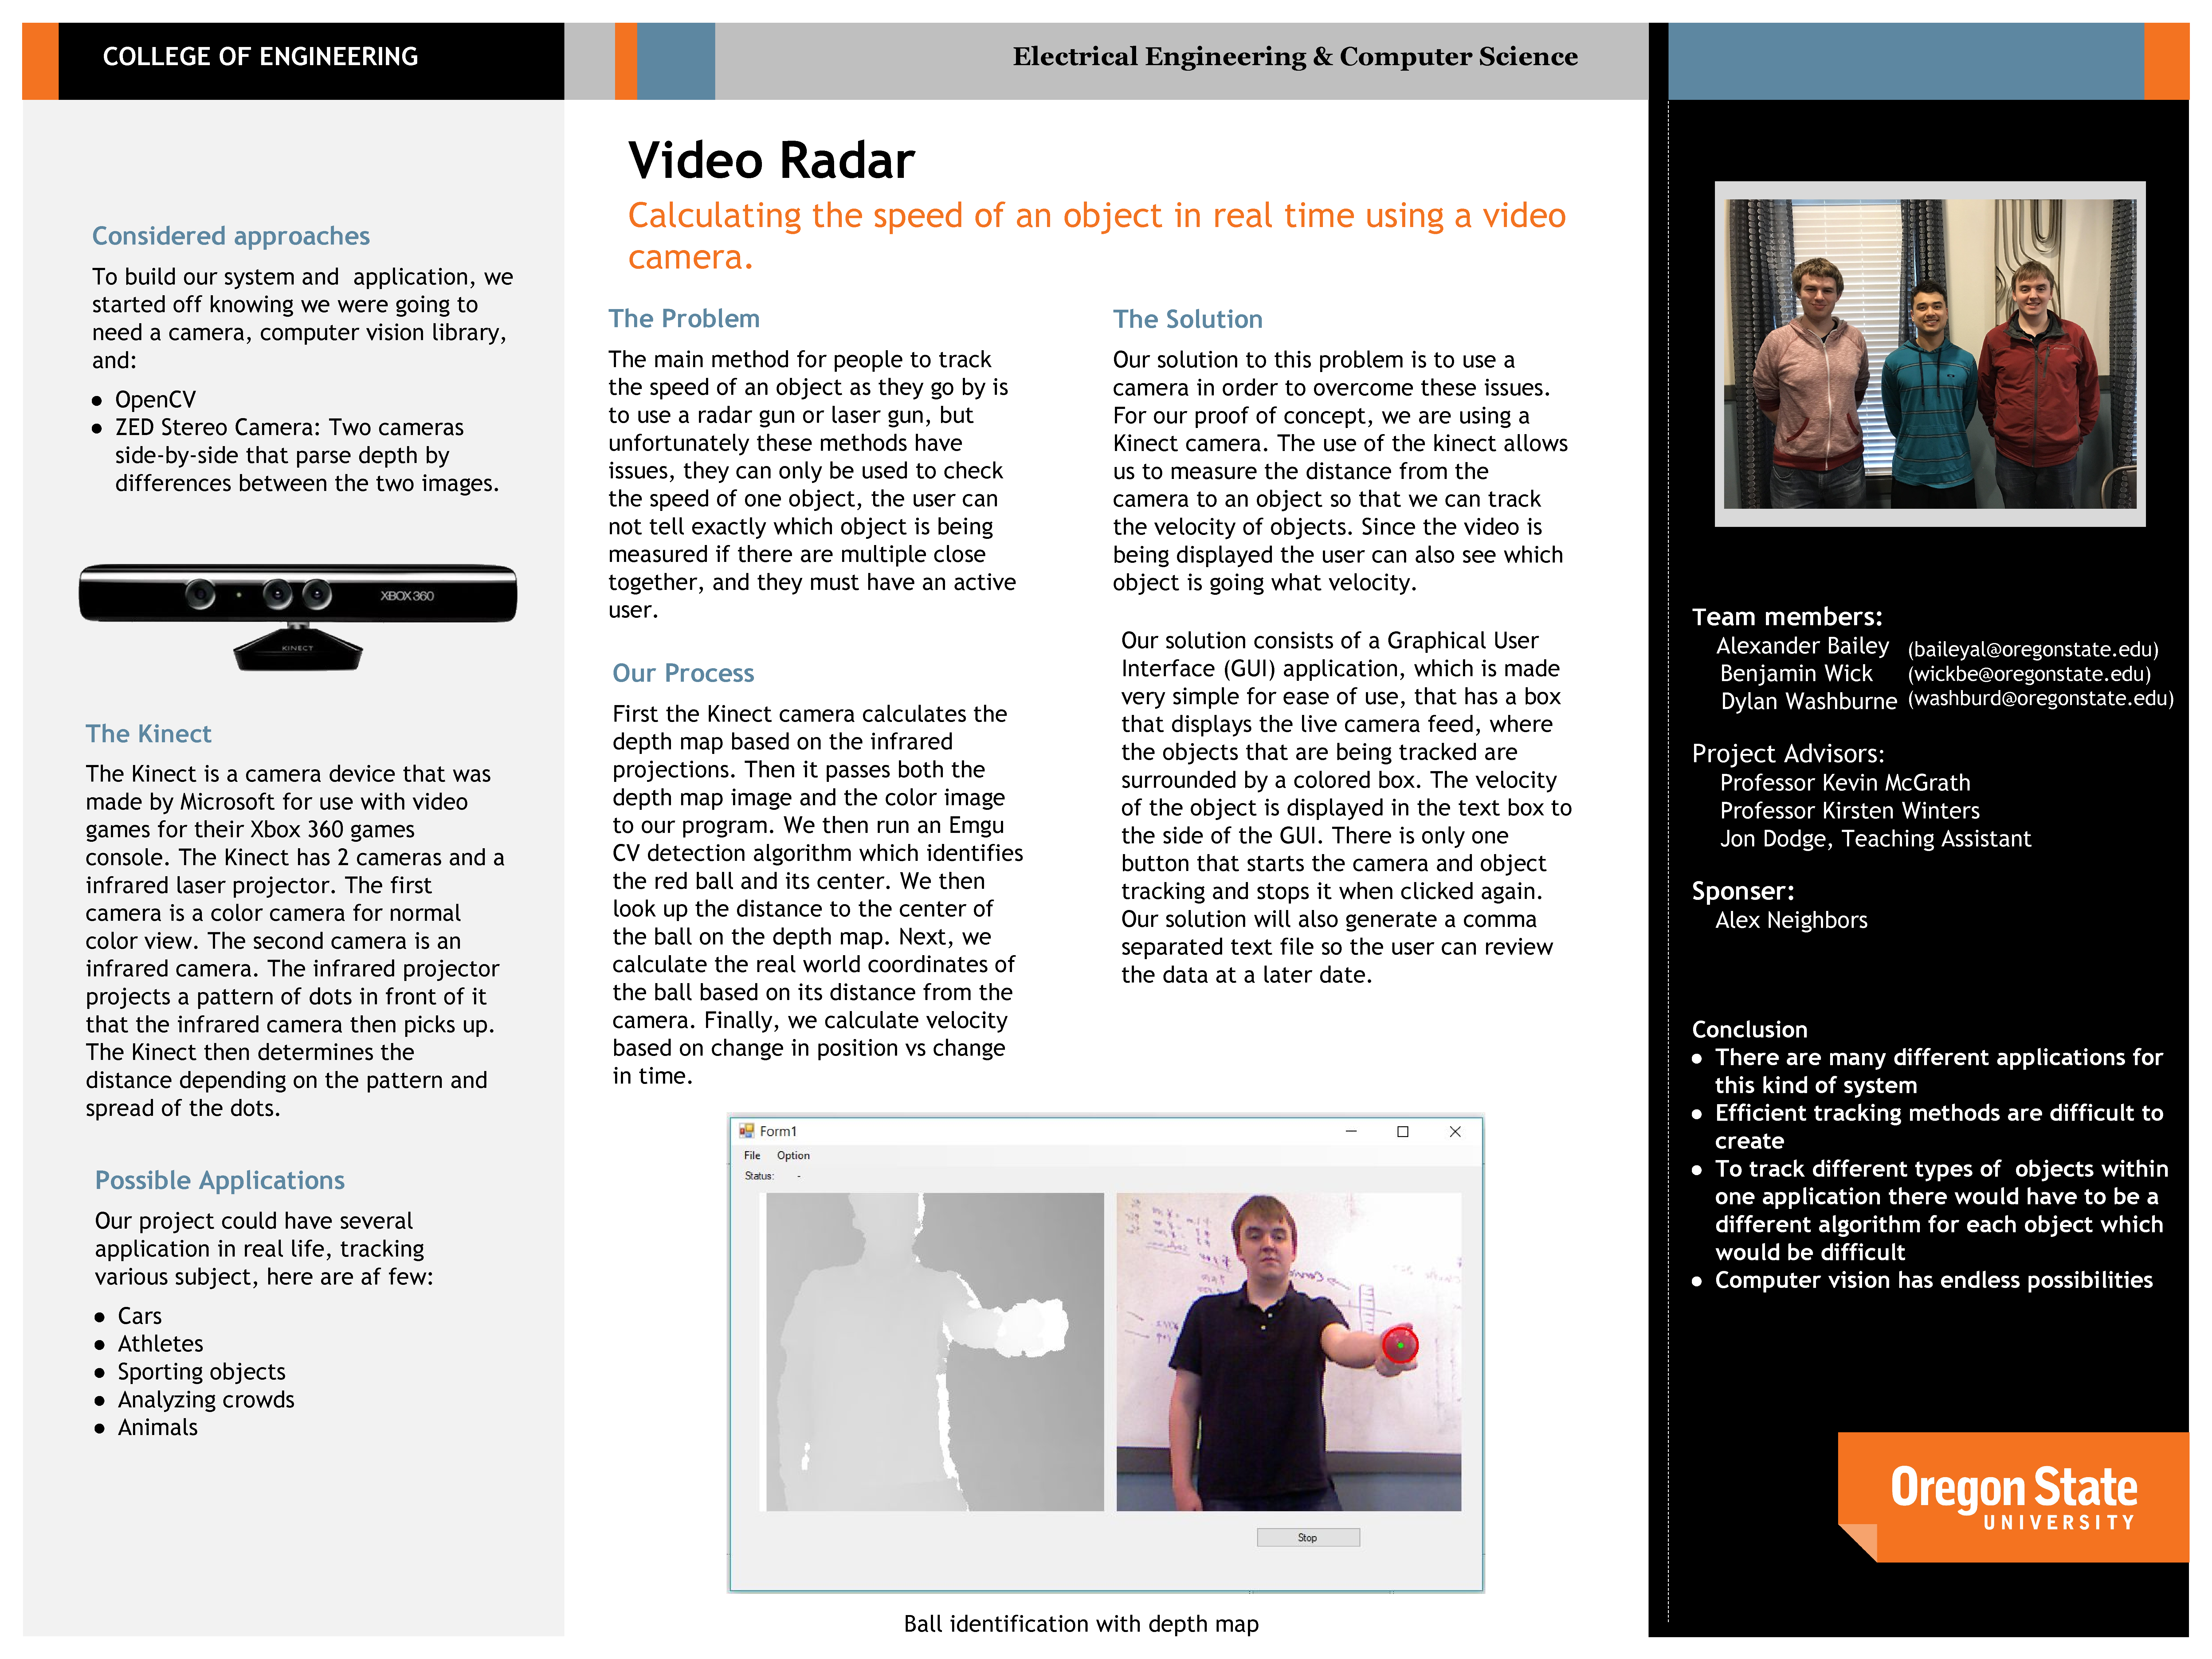
\includepdf[pages={1}]{37_poster.pdf}

\newpage
\section{Project Documentation}

\subsection{How Our Project Works}

Our project is a Windows application.
Our application is developed in C\#, specifically a windows form application.
Our application has a GUI developed using C\#.
In this GUI, we have two image boxes.
The image on the left displays the depth map, while the right box displays the camera image with an overlay to identify the tracked object.
Next there is the text box, which displays the position and speed of the tracked object.
The record button starts and stops the Kinect camera.
For the code, when the window is created, the necessary Kinect variables are initialized.
Then when the start button is pushed, the Kinect is activated.
When the Kinect prepares both the color image and the depth map, the the allFramesReady event is called.
In this event the depth map and color image are transfered to a global variable for later use, calling functions to change the type of image.
Then the processframe function is called.
In this function, we are tracking the red ball.
This is done by finding all the red pixels on the screen by using a range of hue values, which indicate red pixels, that exist for each image.
Once we have all the red pixels we are creating a thresholded image that just shows only the red pixels on the image.
Next we run a few EmguCV calls to filter out outlying pixels to make the thresholded image more accurate and then we are able to draw a circle around the object.
After the object is identified, the speed calculation is inside an if statement that is only entered at a rate less than the camera's speed in order to prevent lag.
Inside of this if statement, the z disposition is determined by reading the depth map and subtracting from the previous frames z value.
The x and y displacements are then calculated by subtracting from the previous frames values and multiplying by the z position in order to compensate for the fact that the further away the object is the smaller it appears.
The speed is then calculated as a displacement of the x, y, z divided by the frame-rate of the camera divided by the tick rate, the rate of reducing the speed calculation.
Finally the depth map and the color image with overlay are copied to the screen and the speed is written to the text box.


\subsection{Setting up our project}
The following is a list of software and the location to download it. All of the following is required to run the project. Included is also the steps to make sure the program compiles correctly.\newline
\textbf{Required Software:}\newline
1. Kinect for Windows SDK v1.8 - https://www.microsoft.com/en-us/download/details.aspx?id=40278
\newline
2. EmguCV library 3.1.0.2504 - https://sourceforge.net/projects/emgucv/
\newline
3. Used for development: Visual studio 2015 community version (.dll is specified for this version)
\newline
\textbf{Steps to compile:}\newline
1. Install Kinect SDK v1.8\newline
2. Install EmguCV library v 3.1.0.2504 and set up environment

(a) Set system environment variable path to C:\textbackslash Emgu\textbackslash emgucv-windesktop 3.1.0.2504\textbackslash bin\textbackslash x86
\newline
3. Open the project solution with Visual Studio and run

\subsection{Hardware Required}
We chose to use the Microsoft Xbox 360 Kinect. The Kinect has an RGB camera as well as two 3D depth sensors. These depth sensors should help us create a depth map that can be used to determine the distance of a person on the screen, which will be vital in determining speed.
\newline
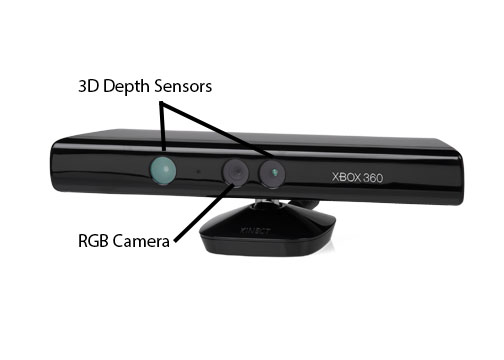
\includegraphics[height=5.5cm]{kinect1.jpg}
\newline
The Kinect was made for the Xbox 360 which meant we had to buy an adapter that will allow us to plug it into a female USB port. Below is an image of the adapter that will be used to do so.
\newline
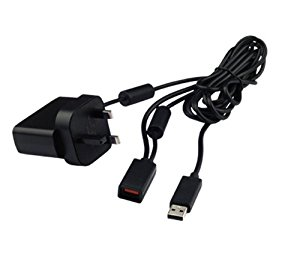
\includegraphics[height=5.5cm]{adapter.jpg}
\newline
Both these hardware components aren't necessary for every system to be implemented.
Theoretically, other cameras may be used depending on the object being tracked.
We chose to use the Kinect because of price, convenience, and the ability to detect people.
The combination of these two hardware pieces will allow us to create a live video for our program to detect objects which will help us obtain our goal.



\section{Learning New Technology}
Our team knew very little about the technology that we were going to be using coming into the project. This meant we had to do tons of research about the Kinect, differnt tracking algorithms using computer vision, as well as the different variables and challenges when trying to calculate the speed of an object using a camera.
This meant our primary resource was Google.
We spent a lot of time researching everything we needed.
The following is a list of main resources we used when researching information.
\begin{itemize}
\item EmguCV documentation - \url{http://www.emgu.com/wiki/index.php/Main_Page}
\item EmguCV code examples - \url{http://www.emgu.com/wiki/index.php/Code_Gallery}
\item StackOverflow forum - \url{https://stackoverflow.com/}
\item MSDN Kinect documentation - \url{https://msdn.microsoft.com/en-us}
\end{itemize}

\section{What We Learned}
This section will go through each individual member of our team and discuss what we learned over the course of the year. Each member will answer specific questions regarding this year.

\subsection{Alexander Bailey}
\subsubsection{What technical information did you learn?}

During this capstone project I learned  about using the Kinect, about the various ways that it could be used, how to use its depth map, about the various functions that is came with.
I also learned about C\# and its similarity and difference to C++.
I learned about using even driven programming.
Up until this point in my computer science career, my programs have been almost entirely programs which followed a set order, first one thing then another then another.
However, with this project, the flow of the program depended largely on human interaction and the flow of the Kinect, as I did not know when the Kinect's data would be ready.
Finally, with this project I gained experience working with a program GUI, designing it to be simple and appealing, as well as the code to handle the button clicks.


\subsubsection{What non-technical information did you learn?}

Working on this project has taught me a lot about how the flow of a project can go.
As this is the first time that I have had to be a part of a large scale project from start to finish.


\subsubsection{What have you learned about project work?}

This project has shown me how much of project is planning and paperwork.
The importance of planning out a project so that future problems can be minimized.
Documentations is also important because there will almost always come a time when the project will be used for someone else and if it is no properly documented, then it will be almost entirely useless or the other party will need to spend a large amount of time digging into the program just to understand how to use it.

\subsubsection{What have you learned about project management?}

During this project I have realized that it is important not to overreach when planning a project, because this can lead to many problems down the read.
It is best to do enough research so that it can be determined how difficult each goal is and how much can be done given the limited time attached to the project.
It is a good idea to set more reasonable goals for a given project and then when those are achieved, to take the project a step further.

\subsubsection{What have you learned about working in teams?}

I have learned that is important to meet as a group on a regular basis in order to make sure that everyone is on the same page.
Meeting regularly also helps to keep everyone on task and motivated.
It is also a good idea to set group goals, giving everyone something to strive for in the immediate future.

\subsubsection{If you could do it all over, what would you do differently?}

If I could do this project over, the main thing I would do is to have a more realistic goal, as our original design document was too much.
I would also make sure that we met at least twice a week, possible more as well as setting very specific weekly goals in order to make sure that we were making good progress.


\subsection{Dylan Washburne}
\subsubsection{What technical information did you learn?}
This project taught me about the software development cycle in general, as though I have held programming positions in the past, I have never been a core part of the design teams, nor have I even had nearly as much power in the building process.  While historically I have been assigned to maintain and implement additional features, the act of creating a piece of software from nothing is an entirely new and unique challenge to me.  I learned about computer vision, C\#, repo management, and to a lesser degree, a number of features of Visual Studio.

\subsubsection{What non-technical information did you learn?}
On the non-technical side, I have learned about some more basic management techniques, though this was never expressly taught and the act of managing was shared among everyone on the team.  I also learned about the act of writing documents which lay out the expectations of the project, and how to properly interact with the client throughout the entire process.

\subsubsection{What have you learned about project work?}
I learned how much work is actually done in the planning and preparation steps.  I have never before had to so precisely document all possible outcomes associated with building a project before building any part of it, but I must say that having so precisely mapped out what I wanted to be done, it certainly streamlined steps later.  That said, I also learned how to properly assess work loads associated with individual tasks, as my estimates were way off.

\subsubsection{What have you learned about project management?}
I have learned that projects don't necessarily need to have a team leader, however it is beneficial to delegate actions to people so there is a sense of direction to pursue.  In fact, I'd say that simply having some objectives available to be completed is the most important part, because then people can simply pick an objective and pursue it.

\subsubsection{What have you learned about working in teams?}
Teams are really just a group of people who should (at least in theory) be pursuing a common goal between all of themselves.  For longer-term projects, this process is made more convenient when the people can get along and effectively use each other at any given time to optimize the performance of everyone involved.  I don't think we hit that point, but I do think that we have a good rhythm going where we can work efficiently until we see a decrease in performance, where we are able to cut it off and regroup at a later time.  That later time can be in a few minutes or the next day, but the important part is that we got what we needed complete.

\subsubsection{If you could do it all over, what would you do differently?}
I would absolutely have started on every project at least a couple days earlier, and I would have aimed way lower in the requirements documents.  The starting earlier is somewhat self-explanatory, to even out the workloads, but even in the cases where we were fine holding off, I would rather have done a couple pieces per day than create a time crunch.  As for the requirements, that actually stems more from me not wanting to tell the client "we messed up our predictions" more than anything else.  Our client was remarkably accomodating, but I still did not like walking up to him and saying we could not complete what was promised, albeit a bit foolishly promised.


\subsection{Benjamin Wick}
\subsubsection{What technical information did you learn?}
This project has taught me a lot about UI development in visual studios, computer vision, and the Microsoft Kinect. This was my first project where we designed a user interface. Visual studios ended up being a very useful tool when doing this. It made things incredibly easy to design and had the exact tools we needed to create our simple application. I also learned how powerful computer vision can be. When doing research on OpenCV, there were many different example projects ranging from facial recognition to changing and distorting images. I learned how to research and use the OpenCV library to function the way we needed it to. Last but not least, I also learned how the Kinect can be a powerful development tool. The Kinect was capable of things we did not expect including creating a 3D depth image to detect how far objects are in relation to the camera.

\subsubsection{What non-technical information did you learn?}
One valuable thing I learned from this project is the ability to go out and research information on my own. This is a valuable skill that can be easily used in the future on the job. I also learned about the process of project development as well as the client and developer interaction aspect. I learned more about how to write well-written documents that are important to project development.

\subsubsection{What have you learned about project work?}
Specifically I learned that it is really important to plan out and design your project. Having a good plan and design can make the project flow a lot easier during the implementation phase. This means putting in the research needed for your project as well as creating a timeline of what you plan to accomplish.

\subsubsection{What have you learned about project management?}
I learned that creating specific weekly goals that the team intends on accomplishing is incredibly useful. This way it makes the project more manageable and having a set goal gives sense of accomplishment to the team.

\subsubsection{What have you learned about working in teams?}
One thing I learned about working in a team is that dividing and conquering is the best method to accomplishing tasks. We ended up dividing work between our team members which allowed us to easily write the documents and implement things at a faster pace.

\subsubsection{If you could do it all over, what would you do differently?}
If I could go back I would set the requirements lower at the beginning. When we started the project, we kind of had the freedom to set the requirements ourselves as our client told us this was mainly our project. We all had an idea in mind but we did not really know how difficult it was. We ended up having to scale the project back. If I could go back and re-do it, I would set the requirements a little lower and set more difficult sounding tasks as stretch goals or add them later in the project.



\section{Appendix 1}
\begin{lstlisting}[language=java]
void ProcessFrame()
        {
            // Create camera instance
            // originalImage = captureCamera.QueryFrame();

            // Create instances
            hsvImage = new Mat(originalImage.Size, DepthType.Cv8U, 3);
            upper_red_hue_range = new Mat(originalImage.Size, DepthType.Cv8U, 1);
            lower_red_hue_range = new Mat(originalImage.Size, DepthType.Cv8U, 1);
            processedImage = new Mat(originalImage.Size, DepthType.Cv8U, 1);

            // Convert to HSV image
            CvInvoke.CvtColor(originalImage, hsvImage, ColorConversion.Bgr2Hsv);

            // Create range of hue value for red and then add both to the processedImage
            CvInvoke.InRange(hsvImage, new ScalarArray(new MCvScalar(0, 155, 155)), new ScalarArray(new MCvScalar(20, 255, 255)), lower_red_hue_range);
            CvInvoke.InRange(hsvImage, new ScalarArray(new MCvScalar(160, 155, 155)), new ScalarArray(new MCvScalar(179, 255, 255)), upper_red_hue_range);

            CvInvoke.Add(lower_red_hue_range, upper_red_hue_range, processedImage);
            CvInvoke.GaussianBlur(processedImage, processedImage, new Size(3, 3), 0);

            Mat structuringElement = CvInvoke.GetStructuringElement(ElementShape.Rectangle, new Size(3, 3), new Point(-1, -1));

            //CvInvoke.Threshold(processedImage, processedImage, 10, 255, ThresholdType.Binary);
            //CvInvoke.BitwiseAnd(mask, s, mask, null);

            CvInvoke.Dilate(processedImage, processedImage, structuringElement, new Point(-1, -1), 1, BorderType.Default, new MCvScalar(0, 0, 0));
            CvInvoke.Erode(processedImage, processedImage, structuringElement, new Point(-1, -1), 1, BorderType.Default, new MCvScalar(0, 0, 0));

            CircleF[] circles = CvInvoke.HoughCircles(processedImage, HoughType.Gradient, 2.0, processedImage.Rows / 4, 100, 50, 0, 0);

            // Drawing circles around objects
            foreach (CircleF circle in circles)
            {
                CvInvoke.Circle(originalImage, new Point((int)circle.Center.X, (int)circle.Center.Y), (int)circle.Radius, new MCvScalar(0, 0, 255), 2);
                CvInvoke.Circle(originalImage, new Point((int)circle.Center.X, (int)circle.Center.Y), 3, new MCvScalar(0, 255, 0), -1);
            }

            tick--;
            if (circles != null && circles.Length != 0)
            {
                //this.speed_val_label.Text = ((ushort)depth_data[(depth_data_width * (int)circles[0].Center.Y) + ((int)circles[0].Center.X)]>>3).ToString();

                x_pos = (int)circles[0].Center.X;
                y_pos = (int)circles[0].Center.Y;
                z_pos = (ushort)depth_data[(depth_data_width * (int)circles[0].Center.Y) + ((int)circles[0].Center.X)] >> 3;

                double x_disp, y_disp, z_disp;

                if (tick <= 0)
                {

                    if (textBox1.Text != "")
                    {                         // if we are not on the first line in the text box
                        textBox1.AppendText(Environment.NewLine);         // then insert a new line char
                    }

                    textBox1.AppendText("ball position x = " + x_pos.ToString() + ", y = " + y_pos.ToString() + ", z = " + z_pos.ToString());
                    textBox1.ScrollToCaret();             // scroll down in text box so most recent line added (at the bottom) will be shown


                    tick = tick_rate;

                    x_disp = (x_pos - x_prev) * z_pos;  //147*2250 = 310*1097
                    y_disp = (y_pos - y_prev) * z_pos;
                    z_disp = Math.Pow(z_pos - z_prev, 2);  //1 ft = 304.8mm
                    double speed = ((Math.Sqrt(Math.Pow(x_disp, 2) + Math.Pow(y_disp, 2) + Math.Pow(z_disp, 2))) / Math.Pow(304.8, 2) * (30/tick_rate));
					//sqrt(x^2+y^2+z^2) * pixels-to-feet

                    this.speed_val_label.Text = speed.ToString();

                    x_prev = x_pos;
                    y_prev = y_pos;
                    z_prev = z_pos;

                    // write lines of text to the file
                    datafile.WriteLine(x_pos.ToString() + "," + y_pos.ToString() + "," + z_pos.ToString() + "," + speed.ToString());
                }
            }

            imageBox1.Image = originalImage;
            //imageBox2.Image = upper_red_hue_range;
        }

\end{lstlisting}


\section{Appendix 2}


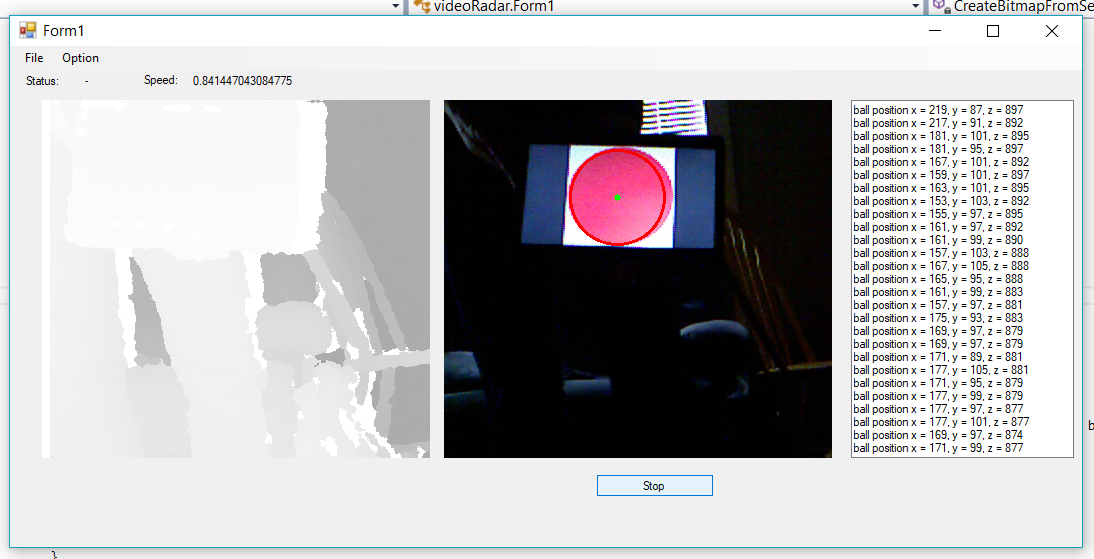
\includegraphics[height=10cm]{projectgui.png}
Here is the final version of our GUI.


\end{document}